%!TEX root = main.tex

\section{Introduction}
\label{sec:introduction}

Supporting modern applications that rely on accurate and real-time analytics  computed over large and continuously evolving databases is a challenging data management problem~\cite{LB:SIGMOD:2015}. Special cases are the classical problems of incremental view maintenance (IVM)~\cite{Chirkova:Views:2012:FTD,DBT:VLDBJ:2014} and stream query processing~\cite{abadi2005design,madden2005tinydb}. 

Recent efforts studied the problem of computing machine learning (ML) tasks over {\em static} databases. The predominant approach loo\-sely integrates the database systems with the statistical packages \cite{MADlib:2012,Rusu:2015,MLlib:JMLR:2016,Polyzotis:SIGMOD:Tutorial:17,Kumar:SIGMOD:Tutorial:17}: First, the database system computes the input to the statistical package by joining the database relations. It then exports the join result to the statistical package for training ML models. This approach precludes real-time analytics due to the expensive export/import steps. 
Systems like Morpheus~\cite{KuNaPa15} and LMFAO~\cite{LMFAO:SIGMOD:2019} push the ML task inside the database and learn ML models over static normalized data. Morpheus decomposes the task of learning generalized linear models into subtasks that are pushed down past a key-foreign key join. LMFAO, and its precursors F~\cite{SOC:SIGMOD:2016} and AC/DC~\cite{ANNOS:TODS:2020}, decompose the task of learning classification and regression models over arbitrary joins into factorized computation of aggregates over joins and fixpoint computation of model parameters. This factorization may significantly lower the complexity by avoiding the computation of Cartesian products lurking within joins~\cite{BKOZ:PVLDB:2013,Olteanu:FactBounds:2015:TODS}. Both the tight integration of the database computation step and of the statistical computation step as well as the factorized computation are pre-requisites for real-time analytics.


This article describes \DF\footnote{\url{https://github.com/fdbresearch/FIVM}.}, a unified approach for maintaining analytics over changing relational data.  We exemplify its versatility in four disciplines: processing queries with group-by aggregates and joins; learning linear regression models using the covariance matrix of the input features; building Chow-Liu trees using pairwise mutual information of the input features; and matrix chain multiplication. 

F-IVM has three main ingredients: higher-order incremental view maintenance (IVM); factorized computation and data representation; and ring abstraction.

The first ingredient allows to reduce the maintenance of a task to that of a hierarchy of simple views. Such views are functions mapping keys, which are tuples of input values, to payloads, which are elements from a task-specific ring. In contrast to classical (first-order) IVM, which computes changes to the query result on the fly and does not use extra views, \DF can tremendously speed up the maintenance task and lower its complexity by using carefully chosen extra views. Nevertheless, \DF can use substantially fewer and cheaper views than the fully-recursive incremental view maintenance approach, which is used by the state-of-the-art IVM system DBToaster~\cite{DBT:VLDBJ:2014}. 

The second ingredient supports efficient computation and representation for keys, payloads, and updates. \DF exploits insights from query evaluation algorithms with best known complexity and optimizations that push aggregates past joins~\cite{BKOZ:PVLDB:2013,Olteanu:FactBounds:2015:TODS,FAQ:PODS:2016}. It can process bulk updates expressed as low-rank decompositions~\cite{TensorDecomp:2009,TensorDecomposition:2017}. It can also maintain compressed (factorized) representation of query results, which is essential to achieve the best possible complexity for free-connex acyclic and $q$-hierarchical queries.

The third ingredient allows \DF to treat uniformly seemingly disparate tasks. In the key space, all tasks require general joins and variable marginalization. In the payload space, tasks differ in the sum and product ring operations. For maintaining linear regression models and Chow-Liu trees under updates, \DF uses a new ring that captures the maintenance of a covariance matrix over continuous and categorical features from the input database. Furthermore, the composition of rings is essential to capture the data-dependent computation for complex analytics. Thanks to the abstraction provided by the ring, \DF is highly extensible: efficient maintenance for new analytics over relational databases is readily available as long as they come with appropriate sum and product ring operations.

\DF is implemented on top of DBToaster's open-source backend, which can generate optimized C++ code from high-level update trigger specifications. In a range of applications, \DF outperforms DBToaster and classical first-order IVM by up to two orders of magnitude in both time and space.

\DF was introduced in a conference paper~\cite{FIVM:SIGMOD:2018}. This article extends and complements that work as follows. Section~\ref{sec:query_classes} introduces an \DF approach that achie\-ves the best known complexities for the well-known classes of free-connex acyclic queries and $q$-hierarchical queries. Section~\ref{sec:applications} introduces the covariance matrix ring, which generalizes the degree-$n$ matrix ring introduced in prior work~\cite{FIVM:SIGMOD:2018} to both continuous and categorical features. Section~\ref{sec:experiments} extends the experiments reported in prior work. It includes new experiments on maintaining: the covariance matrix for continuous and/or categorical features; end-to-end linear regression models; Chow-Liu trees using mutual information; and $q$-hierarchical queries with eager and lazy approaches and payloads carrying the listing or the factorized representation of the query result.


\subsection{F-IVM by Example}
\label{ex:sql_sum_aggregate_intro}

Consider the following SQL query over a database $\db$ with relations $R(A,B)$, $S(A,C,E)$, and $T(C,D)$:
\begin{lstlisting}[language=SQL, mathescape, columns=fullflexible]
  Q := SELECT A,$\;$C,$\;$SUM(B$\,$*$\,$D$\,$*$\,$E) 
       $\,$FROM   R NATURAL$\;$JOIN S NATURAL$\;$JOIN T
       $\,$GROUP$\;$BY A,$\;$C;
\end{lstlisting}
%
Let us consider two different evaluation strategies for this query. 
A na\"{i}ve approach first computes the join result and then the aggregate. This can take time cubic in the size of $\db$.
% 
An alternative strategy exploits the distributivity of the {\tt SUM} operator over multiplication to partially push the aggregate past joins and later combine these partial aggregates to produce the query result. For instance, one such partial sum over $S$ can be expressed as the view V$_\texttt{S}$:
\begin{lstlisting}[language=SQL, mathescape, columns=fullflexible]
  V$_\texttt{S}$ := SELECT A,$\;$C,$\;$SUM(E)$\;$AS$\;$S$_\texttt{E}$ 
        $\,$FROM S GROUP$\;$BY A,$\;$C;
\end{lstlisting}
% 
In the view V$_\texttt{S}$, we identify keys, which are tuples over $(A,C)$, and payloads, which are aggregate values S$_\texttt{E}$. 
Similarly, we compute partial sums over \texttt{R} and \texttt{T} as views V$_\texttt{R}$ and V$_\texttt{T}$. These views are joined as depicted by the {\em view tree} in Figure~\ref{fig:view_tree_sql}, which is akin to a query plan with aggregates pushed past joins. This view tree computes the result of $Q$ in time linear in the size of $\db$.

\begin{figure}[t]
  \centering   
  \includegraphics[width=0.6\columnwidth]{ViewTreeDelta5}
  % \vspace{-2em}
  \caption{View tree for the query in Example~\ref{ex:sql_sum_aggregate_intro}. The propagation paths for updates to $S$ (right red) and to $T$ (left blue).}
  \label{fig:view_tree_sql}
\end{figure}

Consider the problem of learning a linear function $f$ with parameters $\theta_{0}$, $\theta_{D}$ and $\theta_{E}$ that predicts the label $B$ given the features $D$ and $E$, where the training dataset is the natural join of our relations:
\begin{align*}
f(D, E) = \theta_{0} + \theta_{D} \cdot D + \theta_{E} \cdot E
\end{align*}
Our insight is that the same above view tree can also compute the gradient vector used for learning $f$. The only needed adjustment is the replacement of the SQL \texttt{SUM} and \texttt{*} operators with appropriate new sum and product operators. We next explain the case of one model $f$ for each pair of values $(A,C)$; the case of one model for the entire dataset is similar. 

As detailed in Section~\ref{sec:application-lr}, the gradient of the square loss objective function requires the computation of three types of aggregates: the scalar $\LRringC$ that is the count aggregate \texttt{SUM(1)}; the vector $\LRringS$ of linear aggregates \texttt{SUM(B)}, \texttt{SUM(D)}, and \texttt{SUM(E)}; and the matrix $\LRringQ$ of quadratic aggregates \texttt{SUM(B*D)}, \texttt{SUM(B*E)}, \texttt{SUM(D*D)}, \texttt{SUM(D*E)}, and \texttt{SUM(E*E)}. These aggregates are sufficient to capture the correlation between the features and the label.
If we compute them  over each $(A,C)$ group, then we learn one model for each such group; if we compute them over the entire dataset, we learn one model only. 

We treat these aggregates as one compound aggregate $(\LRringC,\LRringS,\LRringQ)$ so we can share computation across them. This compound aggregate can be partially pushed past joins similarly to the SUM aggregate discussed before. Its values are carried in the payloads of keys of the views in the view tree from Figure~\ref{fig:view_tree_sql}. For instance, the partial compound aggregate $(\LRringC_\texttt{T},\LRringS_\texttt{T},\LRringQ_\texttt{T})$ at the view V$_\texttt{T}$ computes for each $C$-value the count, sum, and sum of squares of the $D$-values in $T$. Similarly, the partial aggregate $(\LRringC_\texttt{S},\LRringS_\texttt{S},\LRringQ_\texttt{S})$ at the view V$_\texttt{S}$ computes for each pair $(A,C)$ the count, sum, and sum of squares of $E$-values in $S$. In the view V$_\texttt{ST}$ that is the join of V$_\texttt{T}$ and V$_\texttt{S}$, each key $(a,c)$ is associated with the multiplication of the payloads for the keys $c$ in V$_\texttt{T}$ and $(a,c)$ in V$_\texttt{S}$. This multiplication is however different from SQL's \texttt{*} as it works on compound aggregates: The scalar $\LRringC_\texttt{ST}$ is the arithmetic multiplication of $\LRringC_\texttt{T}$ and $\LRringC_\texttt{S}$; the vector of linear aggregates $\LRringS_\texttt{ST}$ is the sum of the scalar-vector products $\LRringC_\texttt{T}\LRringS_\texttt{S}$ and $\LRringC_\texttt{S}\LRringS_\texttt{T}$; finally, the matrix 
$\LRringQ_\texttt{ST}$ of quadratic aggregates is the sum of the scalar-matrix products $\LRringC_\texttt{T}\LRringQ_\texttt{S}$ and $\LRringC_\texttt{S}\LRringQ_\texttt{T}$, and of the outer products of the vectors $\LRringS_\texttt{T}$ and the transpose of $\LRringS_\texttt{S}$ and also of $\LRringS_\texttt{S}$ and the transpose of $\LRringS_\texttt{T}$. Our approach significantly shares the computation across the aggregates: The scalar aggregates are used to scale up the linear and quadratic aggregates, while the linear aggregates are used to compute the quadratic aggregates.

We now turn to incremental view maintenance. \DF operates over view trees. Whereas for non-incre\-mental computation we only materialize the top view in the tree and the input relations, for incremental computation we may materialize additional views to speed up the maintenance task. Our approach is an instance of higher-order delta-based IVM, since an update to one relation may trigger the maintenance of several views. 

Figure~\ref{fig:view_tree_sql} shows the leaf-to-root paths taken to maintain the view result under changes to $\texttt{S}$ and to $\texttt{T}$. For updates $\delta{\texttt{S}}$ to $\texttt{S}$, each delta view $\delta{V_\texttt{S}}$, $\delta{V_\texttt{ST}}$, and $\delta{\texttt{Q}}$, is computed using delta rules:
% 
% \vspace{-0.25em}
\begin{center}
  
\begin{lstlisting}[language=SQL, mathescape, columns=flexible] 
     $\delta$V$_\texttt{S}$ := $\,$SELECT A,$\;$C,$\;$SUM(E)$\;$AS$\;$S$_\texttt{E}$ 
            $\,\,$FROM $\delta$S GROUP$\;$BY A,$\;$C;
    $\;\;\delta$V$_\texttt{ST}\,$:= SELECT A,$\;$C,$\;$SUM(S$_\texttt{D}$$\,$*$\,$S$_\texttt{E}$)$\;$AS$\;$S$_\texttt{C}$ 
            $\,\,$FROM V$_\texttt{T}$ NATURAL JOIN $\delta$V$_\texttt{S}$ GROUP$\;$BY A,$\;$C;
      $\delta$Q := SELECT A,$\;$C,$\;$SUM(S$_\texttt{B}$$\,$*$\,$S$_\texttt{C}$)
            $\,\,$FROM V$_\texttt{R}$ NATURAL JOIN $\delta$V$_\texttt{ST}$ GROUP$\;$BY A,$\;$C;
\end{lstlisting}
\end{center}
% \vspace{-0.25em}
%
The update $\delta{\texttt{S}}$ may consist of both inserts and deletes, which are encoded as keys with positive and respectively negative payloads. In our example, a negative payload is -1 for the SUM aggregate and $(-1, {\bf 0}_{5 \times 1}, {\bf 0}_{5 \times 5})$ for the compound aggregate, where ${\bf 0}_{n \times m}$ is the $n$-by-$m$ matrix with all zero values.

\DF materializes and maintains views depending on the update workload. For updates to all input relations, it materializes each view in the view tree. For updates to \texttt{R} only, it materializes V$_\texttt{ST}$; for updates to \texttt{S} only, it materializes V$_\texttt{R}$ and V$_\texttt{T}$; for updates to \texttt{T} only, it materializes  V$_\texttt{R}$ and V$_\texttt{S}$. \DF takes constant time for updates to \texttt{S} and linear time for updates to \texttt{R} and \texttt{T}; these complexities are in the number of distinct keys in the views.
In contrast, the classical first-order IVM computes one delta query per each updated relation and without the use of extra views. It takes linear time for updates to any of the three relations for our example query. The fully-recursive higher-order IVM considers a view tree for each delta query so overall more views, including the view materializing the join of V$_\texttt{R}$ and V$_\texttt{S}$.

The above analysis holds for our query with one SUM aggregate. For the learning example with the nine SUM aggregates, \DF still needs the same views. Classical first-order IVM algorithms needs to compute a distinct delta query for each of the nine aggregates -- nine in total for updates to any of the three relations. DBToaster, which is the state-of-the-art fully recursive IVM, computes 28 views, nine top views and 19 auxiliary ones. Whereas \DF shares the computation across the nine aggregates, the classical IVM approach and DBToaster do not. This significantly widens the performance gap between \DF and its competitors.



%%%%%%%%%%%%%%%%%%%%%%%%%%%%%%%%%%%%
\nop{

{\bf One framework to rule them all.}
The generality of our framework stems from its data model: We consider views as functions mapping keys, which are tuples over input data values, to payloads, which represent aggregate values. For instance, $V_R$ contains $A$-values as keys and integer counts as payloads; the input relations are also views that map each tuple to $1$. The example query performs two operations over payloads: when joining two views, the payloads of matching tuples are multiplied, and when computing the {\tt SUM} aggregate, the payloads are added together. 

In this paper, we show how using complex payload types with appropriately defined addition and multiplication can capture various analytical tasks (Section~\ref{sec:applications}). The maintenance procedure remains the same across all tasks for the view keys yet task-dependent for the view payloads. We exemplify this separation of concerns for matrix chain computation, gradient computation for learning linear regression models over joins, and factorized evaluation of conjunctive queries. To support query rewriting such as the above, the set of payload values together with addition and multiplication has to form a semiring or a ring, the latter needed to support IVM with deletions. We define a novel ring that captures the computation of cofactor matrices used in learning regression models over joins and exploit the ring of generalized multiset relations~\cite{Koch:Ring:2010:PODS} to achieve factorized evaluation of conjunctive queries. 

\nop{
Modeling relations as functions, as in previous work~\cite{Koch:Ring:2010:PODS,FAQ:PODS:2016}, enables: 1) a query language that consists of only three operations: unions, joins, and sum aggregates; 2) simplified incremental view maintenance because of simple delta rules that are also expressible using the same query language and without special case distinction of deletions (caused by the non-existence of additive inverse under multiset semantics, $0 + (-R) = 0$).
}

Our approach speeds up view maintenance using three orthogonal shades of factorization, briefly described next. 

{\bf Factorized view computation.}
We decompose a query $Q$ into a view tree that plays the role of a query plan as it dictates the join order and which variables are pushed past joins. 
We exploit the conditional independence among query variables to contain the effects of data explosion in join results and achieve efficient factorized computation: 
In our example, given an $A$ value, $B$ values are independent of $C$, $D$, and $E$ values; similarly, given a $C$ value, $D$ values are independent of values for any other variable. These properties mean that, for instance, we can compute over $D$ values for a particular $C$ value once and reuse the result whenever that $C$ value appears with an $A$ value in $S$. 
We capture such conditional independence using a tree of query variables, called a {\em variable order}, which is used in general variable elimination algorithms, including factorized query processing~\cite{Olteanu:FactBounds:2015:TODS,FAQ:PODS:2016}. 
% Each view tree mirrors the structure of one variable order: At each variable $X$ in the order, we define a view that is a join of its child views followed by (optional) elimination of $X$. 


{\bf Factorized updates.}
The second instance where our framework exploits factorization is when dealing with updates that can be factorized akin to low-rank decomposition of tensors or multi-dimensional matrices. For instance, suppose the update $\delta{S}$ in our example is expressed as a Cartesian product of three smaller deltas: $\delta{S}(A,C,E) = \delta{S_A}(A) \times \delta{S_C}(C) \times \delta{S_E}(E)$. 
This decomposition of $\delta{S}$ breaks the dependency among the query variables $A$, $C$, and $E$, which enables more efficient propagation of updates in the view tree. 
By keeping each of the delta views, $\delta{V_{S}}$, $\delta{V_{ST}}$, and $\delta{Q}$ in the same factorized form -- as a product of expressions -- view maintenance with factorized updates can be asymptotically faster than that with deltas in the listing representation (Section~\ref{sec:factorizable_updates}).

Factorizable updates arise in many domains such as linear algebra and machine learning, where they can represent, for instance, updates to one row/column of a matrix. Section~\ref{sec:applications} shows how our framework can be used for the incremental evaluation of matrix chain multiplication, generalizing prior work~\cite{NEK:SIGMOD:2014}. 


{\bf Factorized payloads.}
Our framework supports view payloads from an arbitrary (semi-)ring. 
In the third instance of factorization in our framework, view payloads are relations (instead of integers like in the above example), which form a ring via appropriately defined addition (union) and multiplication (join). Such relational payloads allow computation and maintenance of results of conjunctive queries in both listing and factorized representations. The latter can be arbitrarily smaller than the former, while still offering constant-delay enumeration of the tuples in the query result~\cite{Olteanu:FactBounds:2015:TODS}.

{\bf Performance.}
We implemented our approach in DBToaster~\cite{DBT:VLDBJ:2014}, which uses program synthesis to generate high-performance maintenance code. The code represents an in-memory standalone stream processor. Armed with our triple lock factorization benefits, \DF clearly outperforms classical first-order IVM, DBToaster's fully recursive higher-order IVM, and plain recomputation by orders of magnitude while using less memory. 

{\bf Complexity analysis.}
Different variable orders may lead to different complexities in our running example. In Appendix~\ref{appendix:complexity}, we analyze the complexity of our approach and introduce a new parameter called the {\em dynamic factorization width}, which connects to known complexity width measures for join queries.
}

\nop{
We make the following contributions:
\begin{itemize}

\item We introduce a higher-order incremental view maintenance (IVM) mechanism for aggregate computation over arbitrary equi-join queries. It relies on an order of the query variables to create a tree of interrelated, factorized views that decompose the query and aggregates.

\item We introduce a framework for incremental computation of various analytical tasks. We define a novel ring that captures the computation of cofactor matrices used in learning regression models over joins (distinct from online learning over a single relation). We exploit the ring of generalized multiset relations to capture factorized evaluation of conjunctive queries. 

\item We build upon three distinct factorization ideas: 1) Factorization of keys exploits conditional independence among query variables to avoid large intermediate join results; 2) Factorization of updates allows more efficient view maintenance when updates are decomposed as sums of products of smaller relations; 3) Factorization of payloads enables expressing conjunctive query results in a factorized form, which can be exponentially more succinct than the listing (flat) representation.

\item Our IVM mechanism can support various aggregate data rings. In particular, we introduce a ring that captures cofactor matrices over factorized joins, which is used for learning linear regression models.

\item We implemented \DF in DBToaster, which uses recursive delta processing and program synthesis to generate high-performance
maintenance code. The experimental results show that our approach can outperform fully recursive and first-order IVM by orders of magnitude while using less memory.

\item In the appendix, we capture the complexity of our IVM mechanism by a new parameter called the dynamic factorization width, which draws on connections to widths for join queries.
\end{itemize}
}


%%%%%%%%%%%%%%%%%%%%%%%%%%%%%%%%%%%%%%%%%%%%%%%%

\nop{
%%%%%%%%%%%%%%%%%%%%%%%%%%%% Figure: Database, Variable order, Factorized join, View tree
\begin{figure*}[t]
\hspace{0.2mm}
\subfloat[Database $\db$]
{
  \label{fig:example_intro_database}
  \begin{minipage}[b]{2.75cm} 
    % \hspace*{-3mm}
    \scalebox{0.92}{
      \begin{tabular}{@{}l@{~~}l@{~$\to$~}l@{}}
        $A$ & $B$ & $\VIEW{R}[A,B]$\\\toprule
        $a_1$ & $b_1$ & $r_1$ \\
        $a_1$ & $b_2$ & $r_2$\\  
        $a_2$ & $b_3$ & $r_3$\\
        $a_3$ & $b_4$ & $r_4$\\\bottomrule
      \end{tabular}
    }
    \\[4ex]
    % \hspace*{-3mm}
    \scalebox{0.92}{
      \begin{tabular}{@{}l@{~~}l@{~~}l@{~$\to$~}l@{}}
        $A$ & $C$ & $E$ & $\VIEW{S}[A,C,E]$ \\\toprule
        $a_1$ & $c_1$ & $e_1$ & $s_1$\\
        $a_1$ & $c_1$ & $e_2$ & $s_2$\\
        $a_1$ & $c_2$ & $e_3$ & $s_3$\\
        $a_2$ & $c_2$ & $e_4$ & $s_4$\\\bottomrule
      \end{tabular}
    }
    \\[4ex]
    % \hspace*{-3mm}
    \scalebox{0.92}{
    \begin{tabular}{@{}l@{~~}l@{~$\to$~}l@{}}
      $C$ & $D$ & $\VIEW{T}[C,D]$ \\\bottomrule
      $c_1$ & $d_1$ & $t_1$\\
      $c_2$ & $d_2$ & $t_2$\\
      $c_2$ & $d_3$ & $t_3$\\
      $c_3$ & $d_4$ & $t_4$\\\bottomrule
    \end{tabular}
    }
    \vspace{1ex}
  \end{minipage}
}
\quad
%
\subfloat[Variable order $\omega$]
{
  \label{fig:example_intro_varorder}
  \begin{minipage}[b]{3cm}
    \centering
    \hspace*{-2mm}
    \begin{small}
      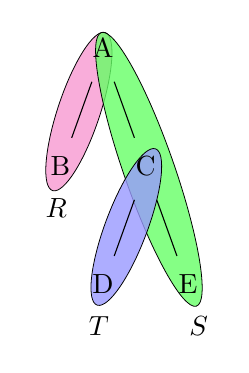
\begin{tikzpicture}[xscale=0.54, yscale=0.5]

        \draw[rotate=73,line width=0.1mm,fill opacity=0.8,fill=magenta!40] (-2.6,-0.2) ellipse (2.1cm and 0.5cm);

        \draw[rotate=-72.2,line width=0.1mm,fill opacity=0.8,fill=green!60] (4.15,-0.2) ellipse (3.65cm and 0.6cm);

        \draw[rotate=71,line width=0.1mm,fill opacity=0.8,fill=blue!40] (-5,-2.3) ellipse (2.1cm and 0.5cm);

        \node at (0, -1) (A) {\phantom{\{}A\phantom{\}}};
        \node at (-1, -4) (B) {\phantom{\{}B\phantom{\}}} edge[-, shorten >=0.1cm, shorten <=0.1cm] (A);
        \node at (1, -4) (C) {\phantom{\{}C\phantom{\}}} edge[-, shorten >=0.1cm, shorten <=0.1cm] (A);
        \node at (0, -7) (D) {\phantom{\{}D\phantom{\}}} edge[-, shorten >=0.1cm, shorten <=0.1cm] (C);
        \node at (2, -7) (E) {\phantom{\{}E\phantom{\}}} edge[-, shorten >=0.1cm, shorten <=0.1cm] (C);
        
        \node at (-1.1, -5) {\normalsize $\VIEW{R}$};
        \node at (-0.1, -8) {\normalsize $\VIEW{T}$};
        \node at (2.25, -8) {\normalsize $\VIEW{S}$};

      \end{tikzpicture}%
      \\[2ex]
      \hspace*{-2mm}
      \scalebox{1} {
        \begin{tabular}{@{~~}l}
          $dep(A) = \emptyset$\\[1ex]
          $dep(B)=\{A\}$\\[1ex]
          $dep(C)=\{A\}$\\[1ex]
          $dep(D)=\{C\}$\\[1ex]
          $dep(E)=\{A,C\}$\\[8ex]
        \end{tabular}
      }
    \end{small}
    \vspace{-3ex}
  \end{minipage}
}
%
\nop{
\subfloat[Factorized join over $\omega$]
{
  \label{fig:example_intro_factorization}
  \begin{minipage}[b]{5.75cm}
    \centering
    \begin{small}
      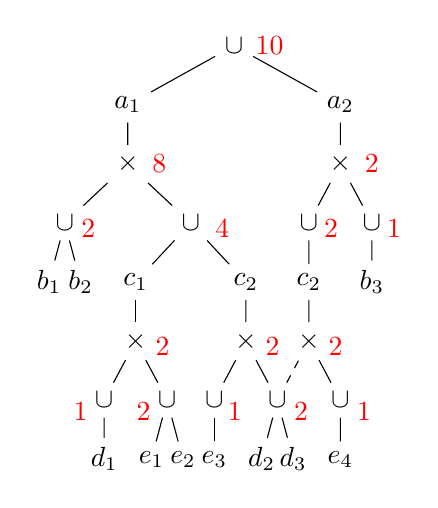
\begin{tikzpicture}[xscale=0.2, yscale=0.75]

        \node at (2.25, 0) (U0) {$\cup$};
        
        \node at (-4.5, -1) (A1) {$a_1$} edge[-] (U0);
        \node at (9, -1) (A2) {$a_2$} edge[-] (U0);
        
        \node at (-4.5, -2) (P1) {$\times$} edge[-] (A1);
        \node at (9, -2) (P2) {$\times$} edge[-] (A2);

        \node at (-8.5, -3) (U1) {$\cup$} edge[-] (P1);
        \node at (-0.5, -3) (U2) {$\cup$} edge[-] (P1);
        \node at (7, -3) (U3) {$\cup$} edge[-] (P2);
        \node at (11, -3) (U4) {$\cup$} edge[-] (P2);

        \node at (-9.5, -4) (B1) {$b_1$} edge[-] (U1);
        \node at (-7.5, -4) (B2) {$b_2$} edge[-] (U1);
        \node at (-4, -4) (C1) {$c_1$} edge[-] (U2);
        \node at (3, -4) (C2) {$c_2$} edge[-] (U2);
        \node at (7, -4) (C3) {$c_2$} edge[-] (U3);
        \node at (11, -4) (B3) {$b_3$} edge[-] (U4);

        \node at (-4, -5) (P3) {$\times$} edge[-] (C1);
        \node at (3, -5) (P4) {$\times$} edge[-] (C2);
        \node at (7, -5) (P5) {$\times$} edge[-] (C3);

        \node at (-6, -6) (U5) {$\cup$} edge[-] (P3);
        \node at (-2, -6) (U6) {$\cup$} edge[-] (P3);
        \node at (1, -6) (U7) {$\cup$} edge[-] (P4);
        \node at (5, -6) (U8) {$\cup$} edge[-] (P4) edge[dashed] (P5);
        \node at (9, -6) (U9) {$\cup$} edge[-] (P5);
        
        \node at (-6, -7) (D1) {$d_1$} edge[-] (U5);
        \node at (-3, -7) (E1) {$e_1$} edge[-] (U6);
        \node at (-1, -7) (E2) {$e_2$} edge[-] (U6);
        \node at (1, -7) (E3) {$e_3$} edge[-] (U7);
        \node at (4, -7) (D2) {$d_2$} edge[-] (U8);
        \node at (6, -7) (D3) {$d_3$} edge[-] (U8);
        \node at (9, -7) (E4) {$e_4$} edge[-] (U9);

        \node at (-7.5, -6.2) {\color{red}$1$}; 
        \node at (-3.5, -6.2) {\color{red}$2$}; 
        \node at (2.3, -6.2) {\color{red}$1$};
        \node at (6.5, -6.2) {\color{red}$2$};
        \node at (10.5, -6.2) {\color{red}$1$};

        \node at (-2.3, -5.1) {\color{red}$2$};
        \node at (4.7, -5.1) {\color{red}$2$};
        \node at (8.7, -5.1) {\color{red}$2$};

        \node at (-7, -3.1) {\color{red}$2$}; 
        \node at (1.5, -3.1) {\color{red}$4$}; 
        \node at (8.4, -3.1) {\color{red}$2$}; 
        \node at (12.4, -3.1) {\color{red}$1$}; 

        \node at (-2.5, -2) {\color{red}$8$}; 
        \node at (11, -2) {\color{red}$2$}; 

        \node at (4.5, -0.0) {\color{red}$10$}; 

      \end{tikzpicture}%
    \end{small}
    \vspace{1ex}
  \end{minipage}
}
}
\quad
% 
\subfloat[View tree over $\omega$]
{
  \label{fig:example_intro_viewtree}
  \begin{minipage}[b]{4.5cm}
    \hspace*{0.2cm}    
    \begin{small}
    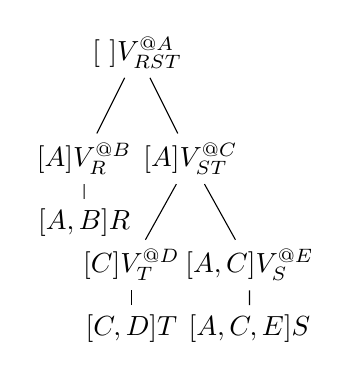
\begin{tikzpicture}[xscale=0.75, yscale=0.27]

      \node at (0.1, 0) (A) {$\VIEW[~]{V^{@A}_{RST}}$};
      \node at (-0.8, -5) (B) {$\VIEW[A]{V^{@B}_{R}}$} edge[-] (A);
      \node at (1, -5) (C) {$\VIEW[A]{V^{@C}_{ST}}$} edge[-] (A);
      \node at (0, -10) (D) {$\VIEW[C]{V^{@D}_{T}}$} edge[-] (C);
      \node at (2, -10) (E) {$\VIEW[A,C]{V^{@E}_{S}}$} edge[-] (C);
      
      \node at (-0.8, -8) {$\VIEW[A,B]{R}$} edge[-] (B);
      \node at (2, -13) {$\VIEW[A,C,E]{S}$} edge[-] (E);
      \node at (0, -13) {$\VIEW[C,D]{T}$} edge[-] (D);

    \end{tikzpicture}
    \end{small}
    \\[6pt]
    \scalebox{0.8}{\parbox{\linewidth}{%
      \begin{align*}
        \VIEW[~]{V^{@A}_{RST}} &= \VSUM_{A} \big(\VIEW[A]{V^{@B}_{R}} \VPROD \VIEW[A]{V^{@C}_{ST}}\big) \\[2pt]
        \VIEW[A]{V^{@C}_{ST}} &= \VSUM_{C} \big(\VIEW[C]{V^{@D}_{T}} \VPROD \VIEW[A,C]{V^{@E}_{S}}\big) \\[2pt]
        \VIEW[A,C]{V^{@E}_{S}} &= \VSUM_{E} \VIEW[A,C,E]{S} \\[2pt]
        \VIEW[C]{V^{@D}_{T}} &= \VSUM_{D} \VIEW[C,D]{T} \\[2pt]
        \VIEW[A]{V^{@B}_{R}} &= \VSUM_{B} \VIEW[A,B]{R} 
      \end{align*}
    }}
    \vspace{4pt}
  \end{minipage}
}
\quad
% 
\subfloat[View keys and payloads]
{
  \label{fig:example_intro_views}
  \begin{minipage}[b]{5cm}
    \hspace*{-0.4cm}    
    \begin{small}
    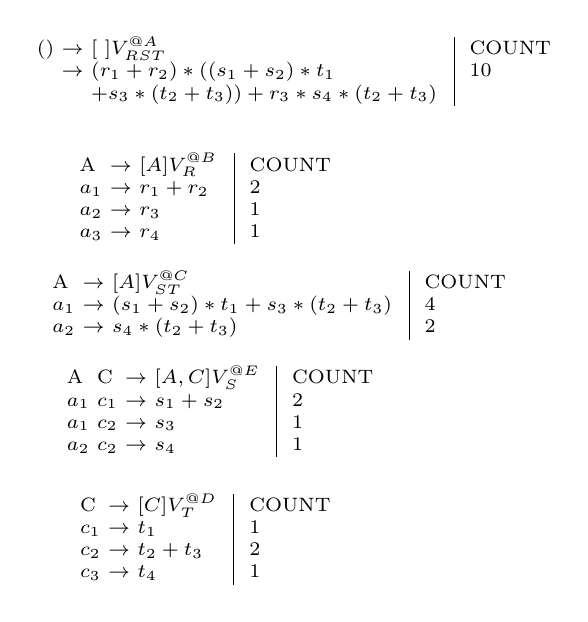
\begin{tikzpicture}[xscale=0.75, yscale=0.27]

      % at node A
      \node at (-5, 8) {
        \scriptsize
        \begin{tabular}{@{}l@{~}l@{~}l|@{~~}l@{}}
          $()$ & $\to$ & $\VIEW[~]{V^{@A}_{RST}}$ & COUNT \\\toprule
          $\tuple{}$ & $\to$ & $(r_1+r_2)*((s_1+s_2)*t_1$ & 10\\
                     &       & $+s_3*(t_2+t_3))+r_3*s_4*(t_2+t_3)$ & \\\bottomrule
        \end{tabular}
      };

      % at node B
      \node at (-6.5, 2) {
        \scriptsize
        \begin{tabular}{@{}l@{~$\to$~}l|@{~~}l@{}}
          % $\VIEW{V^{@A}_R}$ 
          A & $\VIEW[A]{V^{@B}_{R}}$ & COUNT\\\toprule
          $a_1$ & $r_1+r_2$ & 2 \\
          $a_2$ & $r_3$ & 1 \\
          $a_3$ & $r_4$ & 1\\\bottomrule
        \end{tabular}
      };

      % at node C
      \node at (-5.25, -3) {
        \scriptsize
        \begin{tabular}{@{}l@{~$\to$~}l|@{~~}l@{}}
          A & $\VIEW[A]{V^{@C}_{ST}}$ & COUNT\\\toprule
          $a_1$ & $(s_1+s_2)*t_1+s_3*(t_2+t_3)$ & 4 \\
          $a_2$ & $s_4*(t_2+t_3)$ & 2 \\\bottomrule 
        \end{tabular}
      };

      % at node E
      \node at (-6.25, -8) {
        \scriptsize
        \begin{tabular}{@{}l@{~}l@{~$\to$~}l|@{~~}l@{}}
          A & C & $\VIEW[A,C]{V^{@E}_{S}}$ & COUNT\\\toprule
          $a_1$ & $c_1$ & $s_1+s_2$ & 2 \\
          $a_1$ & $c_2$ & $s_3$ & 1 \\
          $a_2$ & $c_2$ & $s_4$ & 1 \\\bottomrule
        \end{tabular}
      };
      
      % at node D
      \node at (-6.5, -14) {
        \scriptsize
        \begin{tabular}{@{}l@{~$\to$~}l|@{~~}l@{}}
          C & $\VIEW[C]{V^{@D}_{T}}$ & COUNT\\\toprule
          $c_1$ & $t_1$ & 1 \\
          $c_2$ & $t_2+t_3$ & 2 \\
          $c_3$ & $t_4$ & 1 \\\bottomrule
        \end{tabular}
      };

    \end{tikzpicture}
    \end{small}
  \end{minipage}
}\vspace*{-1em}

\caption{Database $\db$ with {\color{red}relations} {\color{magenta!80}$\VIEW{R}$}, {\color{goodgreen}$\VIEW{S}$}, {\color{blue!80}$\VIEW{T}$} over some ring $\RING$ such that $\{r_i,s_i,t_i\}_{i\in[4]}\subseteq\RING$. The view payloads are shown over the general ring $\RING$ and also over the $\mathbb{Z}$ ring, where $\forall i\in[4]: r_i=s_i=t_i=1$.}
\label{fig:example_intro}\vspace*{-1em}
\end{figure*}
}

%%%%%%%%%%%%%%%%%%%%%%%%%%%%